\documentclass[11pt]{article}
\usepackage{setspace}
\usepackage{titling}
\usepackage[a4paper,margin=1in]{geometry}
\usepackage{enumitem}
\usepackage{fancyhdr}
\usepackage{titlesec}
\usepackage{ebgaramond}
\usepackage[T1]{fontenc}
\usepackage{hyperref}
\usepackage{graphicx}

\renewcommand{\thesection}{\Roman{section}.}
\renewcommand{\thesubsection}{\alph{subsection}.}
\renewcommand{\thesubsubsection}{\thesubsection\roman{subsubsection}}

% --- header ---
\pagestyle{fancy}
\fancyhf{}
\fancyhead[L]{Department of Computer Science \\
  \rule[-2ex]{0pt}{2ex}Ateneo de Naga University}
\vspace{5cm}
\fancyfoot[C]{\thepage}

\setlength{\headheight}{30pt}
\setlength{\headsep}{20pt}

\begin{document}

% --- cover page ----
\begin{titlepage}
  \thispagestyle{fancy}

  \vspace*{4cm}
  \centering
    \vfill
    {\LARGE \textbf{REVITALISE}} \\
    \vspace{0.5cm}
    CSMC311 Software Engineering 2 \\
    Proposal Paper
    
    \vfill

    \textbf{Game Designer, Programmer, Project Manager} \\
    Jonel C. Ganalon -- N2

    \vspace{1cm}
    
    \vfill 
\end{titlepage}

\section{Introduction}
\subsection{Overview}
Revitalise is a prospective open-source game revolving around the use of languages to reclaim territories overrun by the foreign language of an invading people. It is a turn-based strategy game similar. The player of the game leads the Insurgents aiming to overthrow the foreign government of their land. These insurgents discovered a powerful way to fight the Imperalists using their lost language. They discovered that everything on their land has an original name used before the Imperials arrived. These original names or true names once spoken by native people grant them power on that concept. However, the Imperialists ruined every source of their native language and compels everyone to use their Imperial language. The role of the player comes into play as someone who still has the knowledge of the lost native language. The player must gather allies and teach the people to remember their native language to bring back parts of their culture, identity, and home.


\subsection{Purpose of the Application}
The game has primary and secondary purposes.
\subsubsection{Primary Purpose}
The game provides a platform for documenting languages. The game contains specimens from real-life languages that the player must discover to unlock gameplay elements. Aside from that, players themselves contribute to this purpose by collecting real life words from their chosen language and inputting them into the game. This involves everyone in saving their own languages from possible threats of extinction in the future. This is particularly relevant in the Philippines, where documentation of local languages receives little attention

\subsubsection{Secondary Purpose}
The secondary purpose provides structure on how one can build vocabulary in doing a posteriori constructed languages.


\subsection{Objectives}
Document at least 200 native words in prototype.
Implement turn-based mechanics

\subsection{Game Specifics}
\subsubsection{Game Theme}
Cultural Preservation/Language Revival
Education/Learning
Exploration/Discovery
Identity/Connection
\subsubsection{Game Genres}
Educational
Adventure
Role-playing
\subsubsection{Gameplay and Mechanics}
For the prototype of the game, since Bicol Naga language will be used, the mechanics of the game will revolve around the features of the Bicol Naga langugae. 

The game will be played on a pre-defined map. Players will start at a specific point in the map. They will find themselves already in the company of the Insurgents. The insurgents will tell their story and will ask the players to help to them free their City. Once confirmed, the interface for monitoring the people of the City and the players's ally, the Insurgents, will appear on the screen. The Insurgents are wanted by the Imperial Police, the players must not get caught by them. The players then need to establish their base by using the power of  native words.

The players have HP and Mana attribute. The Mana attribute is consumed when the players are reciting or using words. 

how to increase hp and mana

When the player clicked an antity in the game, a window will appear that lets the player choose between the noun class markers of Bicol. This will make the clicked object as an actor, receiver of an action, or a location of an action.\\

The \textbf{si} set of markers:\\
\textbf{si}: this is used for entities will with personal names such as allies whom the players have given names. This will make the entity the focus of the action. Another usage of \textbf{si} is to refer to entities that has been specified from a given context of conversation. \\
\textbf{an}: Similar to \textbf{si} but is used for common nouns.\\

The \textbf{ni} set of markers:\\
\textbf{ni}: This is used to refer to entities with personal names.\\
\textbf{nin}: This is used to refer to entities that are common or general.\\
\textbf{kan}: This is used to refer to entities that has been specified from a context of conversation.\\

The \textbf{locative} markers refer to a place or direction of an action.\\
\textbf{ki}: This is used for entities with personal names.\\
\textbf{sa}: This is used for entities that has common or general names.\\

At the side panel, list of verbs will appear that the players can use to make an action. Once the players chose an action, a list of possible affixes will show up.

The choices of the players are crucial since this can make an action target the enemy or target themselves or their allies.

Some verbs require another argument to convey different meaning. For example, the verb \textbf{lakaw} can use another argument like \textbf{paduman} in order to convey movement towards something.\\

\textbf{Angry Register}\\
Some words in Bicol have synonimous counterpart that is typically used by its speakers to indicate irration, angriness, or intense emotion. This is called \textbf{angry register} and it is a unique trait of the Bicol language. In the game, these words have stronger effects than the normal ones.\\

\textbf{Food}\\
The players need to secure their source of food. Food recruits people and each people brings one \textbf{Insight} to the players. Insights are necessary in recovering native words and in making new words. The larger the allied people, the more words can be made. The needed number of Insights to create words vary.
Concrete nouns require the least amount of Insights. Next are verbs relating to physical movements. Mental verbs like to think has higher Insight requirements than the normal verbs. Abtracts nouns have high Insight requirement as well.\\

\textbf{Recruitment}\\
The Insurgents are the ones that recruits people. For every insurgent, they collect food and this ables them to recruit people.

\textbf{Insight}
For every people recruited, they add Insight to the players. Every people contributes one Insight. Profesionals offer more Insights.

\textbf{Nouns:}
Every entity in the game has its corresponding nouns. Knowing the nominal names give the players power over that entity. For example, in order to use wood, the player must record the Bicol word kahoy. Nouns reffering to objects have damage attributes. They have varying amount of damage depending on object. For example, sundang has higher damage than tukawan.
There are also nouns referring to places. These nouns can reclaim building institutions in the game like entering the Bicol word for hospital will give players access to it.

Derivation is the process of adding affixes to nouns to create new words. Bicol has several productive ways of doing derivations. Aside from this, players can do neologism. Neologism is where the player creates new word that does not exist in the Bicol language. Doing neologism costs more Insights but sometimes provides additional benefits. It adds more \textbf{prestige} to the language.

The following are the possible \textbf{affixes} in the game:\\


\textbf{Verbs:}
Verbal words give players actions. Learning an action takes time and different actions can have varying needed duration to be learned. Verbs are divided into transitive and intransitive. Transitive verbs require at least two arguments: the actor and the patient; while Intransitive verbs require at least one argument, the actor or the patient.

Conjugation is the adding of affixes to the verb in order to convey mood and aspect.\\

\textbf{Defence}\\
Defence is an attribute that each institutions or buildings has. The defence increase with the number of native words associated to that institution.\\

\textbf{Prestige}\\
Prestige is the meter on how strong the language is. Prestige can be increased with the addition of words into the players' language.\\

\textbf{Combats}\\
There are several combats in the game implemented using turn-based strategy.

\textbf{Physical Objects}
Imperials and the players can fight using physical objects. The damage of the physical object can be increased during fights by using \textbf{semantic chaining}. The enemy or the players provide words related to their weapon. The more words provided, the stronger the attack. This means that bigger vocabulary can offer longer semantic chains.

\textbf{Translations}
The Imperial fights by giving the player a word in English and they must block it by giving the counterpart of word in their language. When the players miss the turn by not knowing the word or giving incorrect word, they will take damage, reducing their HP.

\textbf{Puzzles}
Puzzles are given to the players when they use professionals to become an agent inside a building to steal its Imperial name. If the players succesfully deciphered the puzzle, they can claim the building by naming it. If the players fail to do the puzzle, the professional will be caught and there will be penalties to the players. 




\subsubsection{Story, Setting, and Character}
Many years have passed after the language imperalist Nation conquered every country in the world. Many languages have been lost and the rest nears extinction. No one knows how but one day, these lost languages rise from death and gave its people powers to fight against their colonizers. Few people have discovered this and they form the Insurgents. Their aim is to use this power to reclaim their land and push the Imperials away. They then made their goal to revive their lost native language and cultivate this to protect themselves from foreign invaders. 

The game takes place in an alternate simplified version of Naga City, Camarines Sur, Bicol, Philippines. Since the main purpose of the game is to help preserve languages, it will use real-life languages and copy necessary elements from their origin of place.

\textbf{Professionals} \\
Professionals are allies of the players. They are special people because the players can give them names of profession. Being professionals, they offer higher Insight contribution to the players. Each professional is associated to a building. Professionals then can give the players access inside buildings occupied by the Imperials.



\subsubsection{Levels}
Each institution represents a level. The institutions are associated into one of the eight stages of reviving threantened languages by linguist Fishman.


Family Household
Elementary Schools
Highschools
Colleges
Educational Institutions
Medical Institutions
Religious Institutions
Shopping District
Market
Government, Baranggay, City Hall

the player strengthen the claim of each institution by providing words related to each.

\subsubsection{Interface}

\subsubsection{Map View}
The map is an isometric version inspired by real-life locations in Naga City. It willl be tile-based. Areas controlled by the Imperials will have different color compare to the areas claimed by the players. The map can be moved in up, down, left and right.

\subsubsection{Resource Panel}
\subsubsection{Event and Dialogue Box}
\subsubsection{Control Panels}
\subsubsection{Word History}
This contains the words discovered, created, and used by the players.

\subsubsection{Dictionary}
Players will have their own dictionaries. They are composed of the words that they have entered into the game.

\subsubsection{Technology Tree}

\subsubsection{Combats}



\subsection{Scope and Delimitation}
The protoype of the game will only include a small portion of Naga City and will only use the Bicol language as the native language that the players can choose. English will also be chosen as the foreign language.

The prototype will not include multiplayer support, setting customisations, large-scale maps.



\subsection{Target Audience and Platform}
The game targets people who interests languages may it be as a profession or as a hobby. It also offers itself as a tool to preserve or record real-life languages. Anyone who wants to use their improve their vocabulary on their language and participate in constructing new words can play the game.

The prototype will be made for personal computers.

\subsection{Concept of the Project}
The game takes inspiration from turn-based tactical games like Freeciv and Civilisation. Instead of building a civilisation, the player must retake an already existing society. Similar to the games mentioned, it will also be possible to expand and dominate other player-controlled section of the map. That is one of the visions of the game --- a multiplayer online tactical game.

The game also adopts the concept of technology tree. 

The concept of the game is based from the model of reviving threatened languages by the lingust Joshua Fishman. The model consist of eight stages of using the language. 

\section{TECHNICAL BACKGROUND}
The game will be written using C++, SMFL? 2D
SQL for database

\section{METHODOLOGY}
\subsection{Development Process}
\subsection{Development Process}
The project will adopt an iterative and incremental development process with an emphasis on rapid prototyping. 
Initial efforts will focus on producing quick, playable prototypes to test the core mechanics of the game such as word recovery, resource management, and turn-based progression. 
Feedback from these prototypes will inform successive iterations, where additional features and refinements will be implemented in small increments. 

\subsection{Diagrams}
\url{https://app.diagrams.net/#Lgame%20diagrams.drawio#%7B%22pageId%22%3A%22Ie5LLhRZTwk1cWGMkZ7P%22%7D}

\subsubsection{Use-case Diagram}
\subsubsection{Activity Diagram}
\subsubsection{Data Diagram}

\begin{figure}[h!]
  \centering
  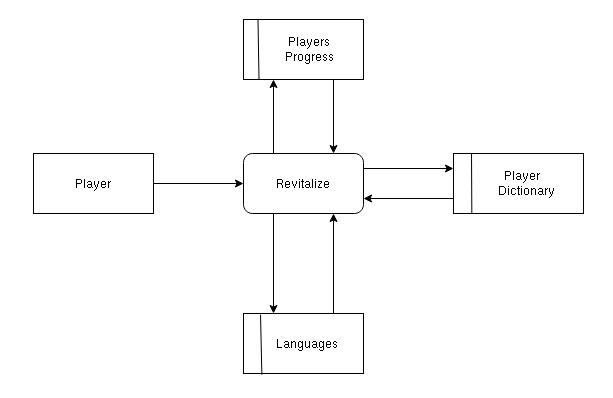
\includegraphics[width=0.7\textwidth]{diagrams/dfd01.png}
  \caption{Level 0 Data flow diagram.}
  \label{fig:dfd0}
\end{figure}

\subsection{Features and Functionalities}
\subsubsection{Food}


\subsection{Timeline and Development Milestones}


\end{document}
